%%%%%%%%%%%%%%%%%%%%%%%%%%%%%%%%
%------------------------------%
%%%%%%%%%%%%%%%%%%%%%%%%%%%%%%%%
\section{Supplementary materials}
%%%%%%%%%%%%%%%%%%%%%%%%%%%%%%%%
%------------------------------%
%%%%%%%%%%%%%%%%%%%%%%%%%%%%%%%%

% 1D LINEAR ADMIXTURE KINSHIP
\begin{figure}[H]
    \centering
    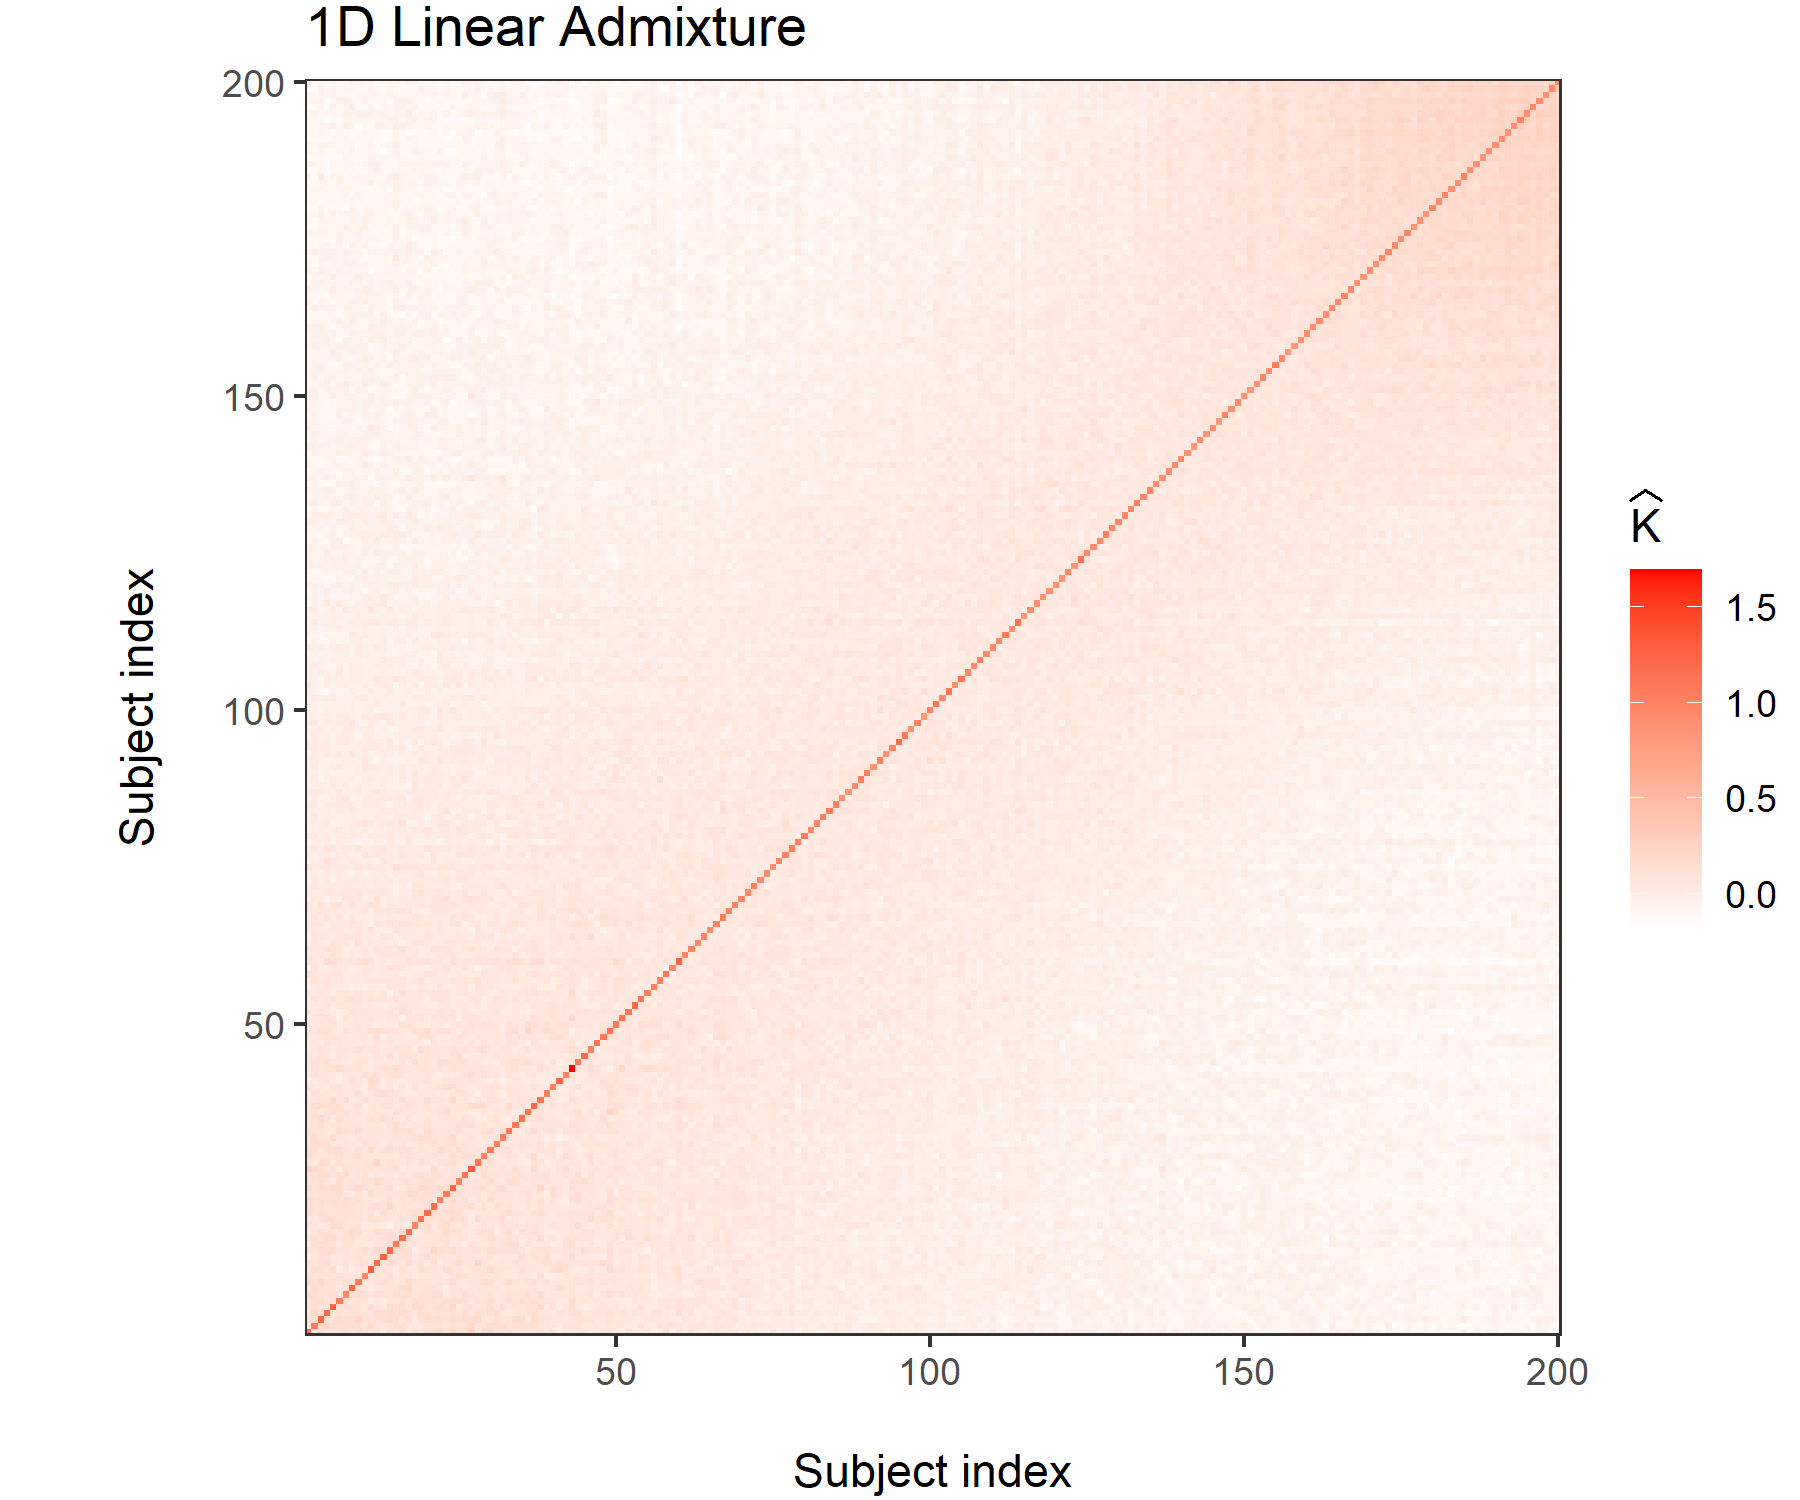
\includegraphics[scale = 1]{figures/admixed_kinship.png}
    \caption{1D Linear Admixture with coarse subpopulation structure (50 subjects per subpopulation), RRM.}
    \label{fig:admixed}
\end{figure}

% INDEPENDENT SUBPOPULATIONS, COARSE, KINSHIP
\begin{figure}[H]
    \centering
    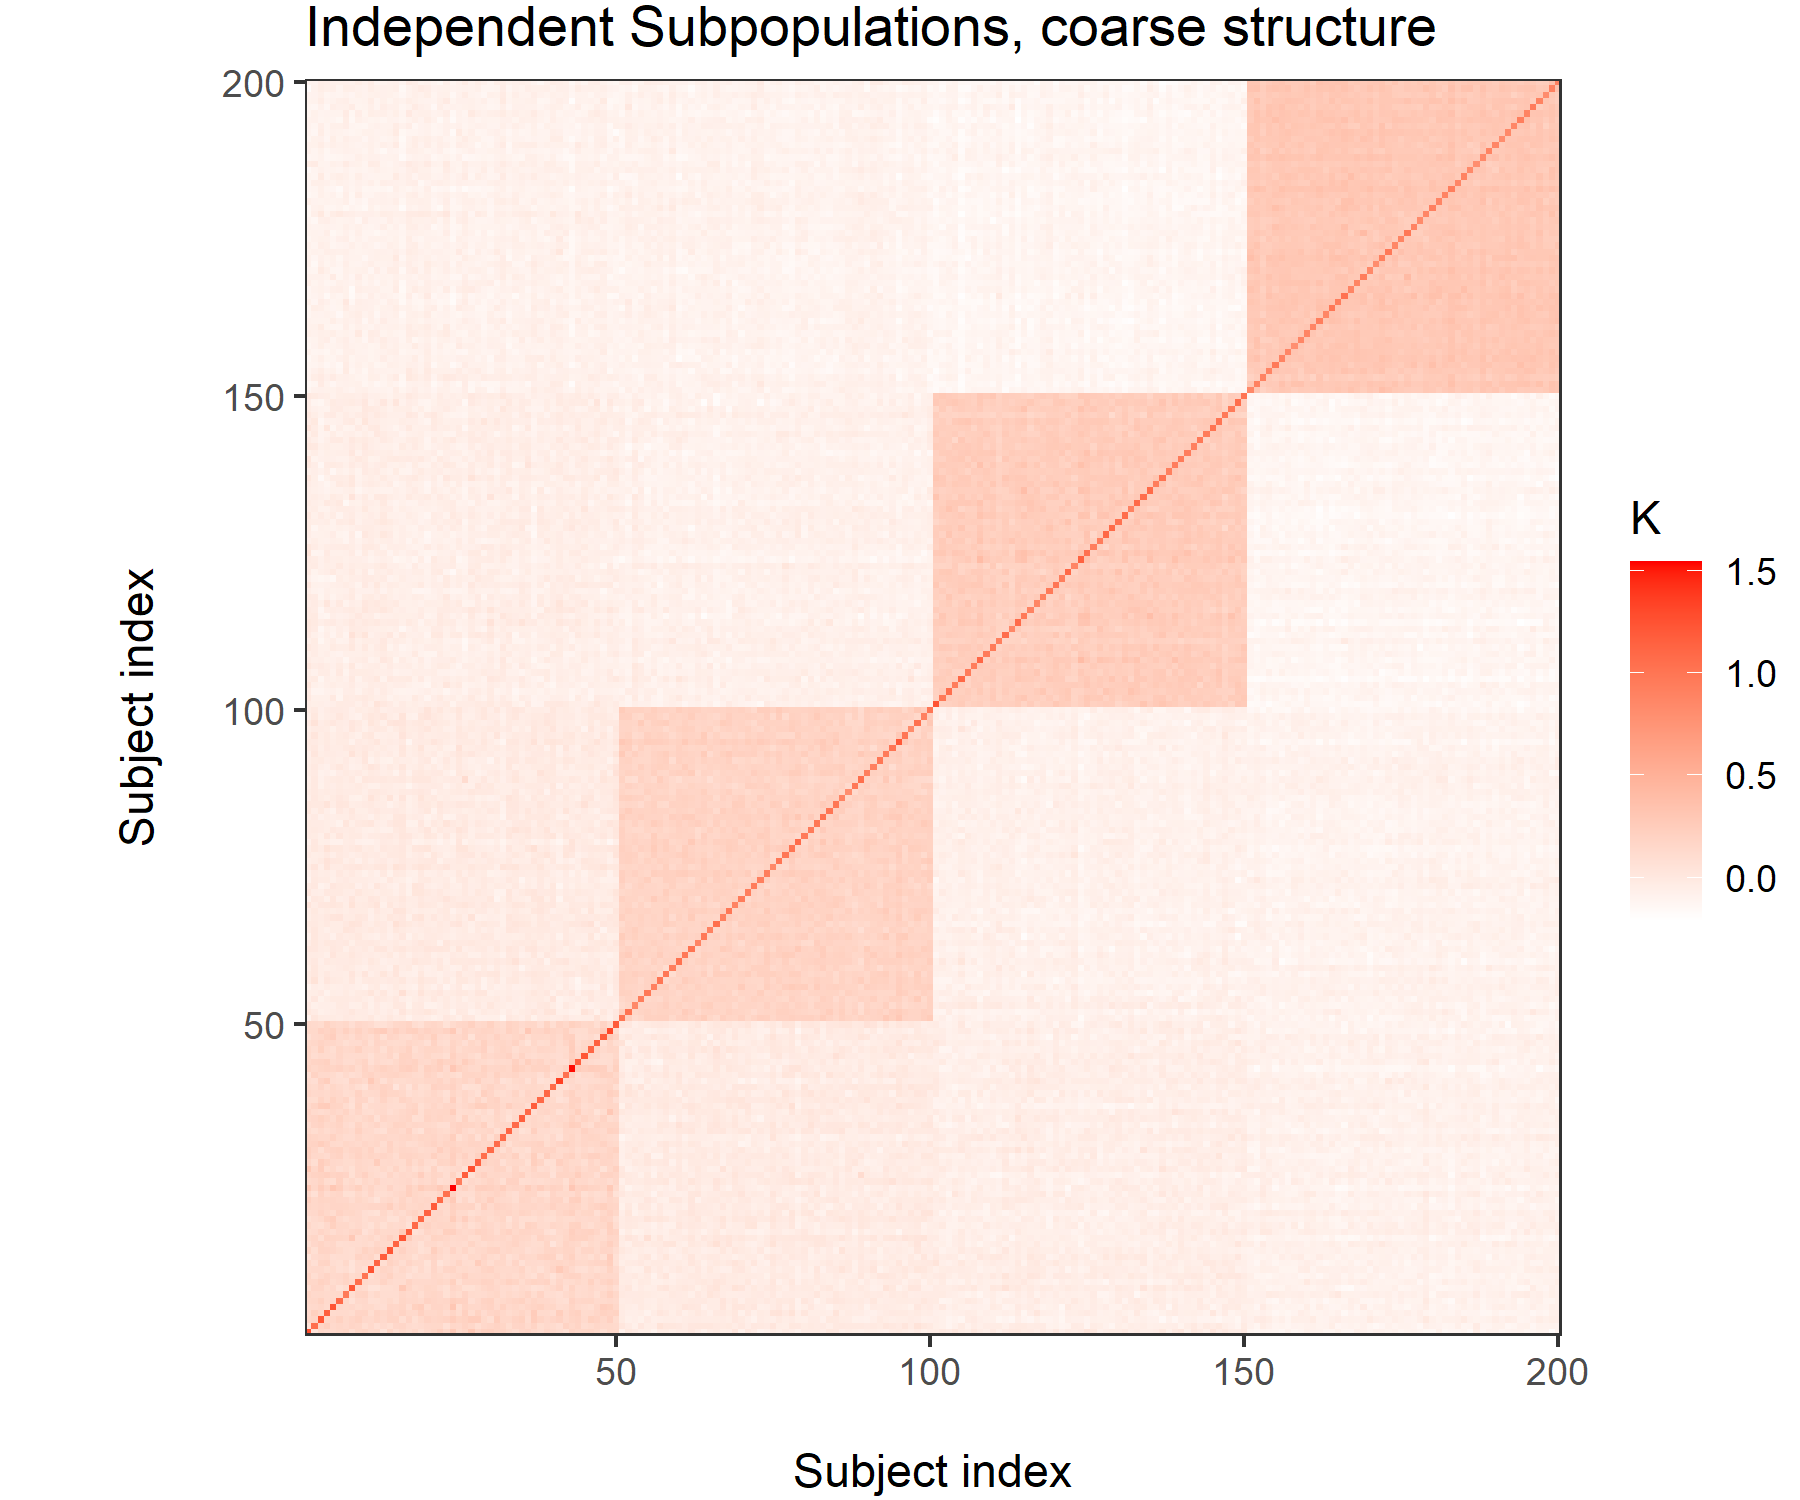
\includegraphics[scale = 1]{figures/indep_coarse_kinship.png}
    \caption{Independent Subpopulations with coarse subpopulation structure (50 subjects per subpopulation), RRM.}
    \label{fig:indep_coarse}
\end{figure}

% INDEPENDENT SUBPOPULATIONS, FINE, KINSHIP
\begin{figure}[H]
    \centering
    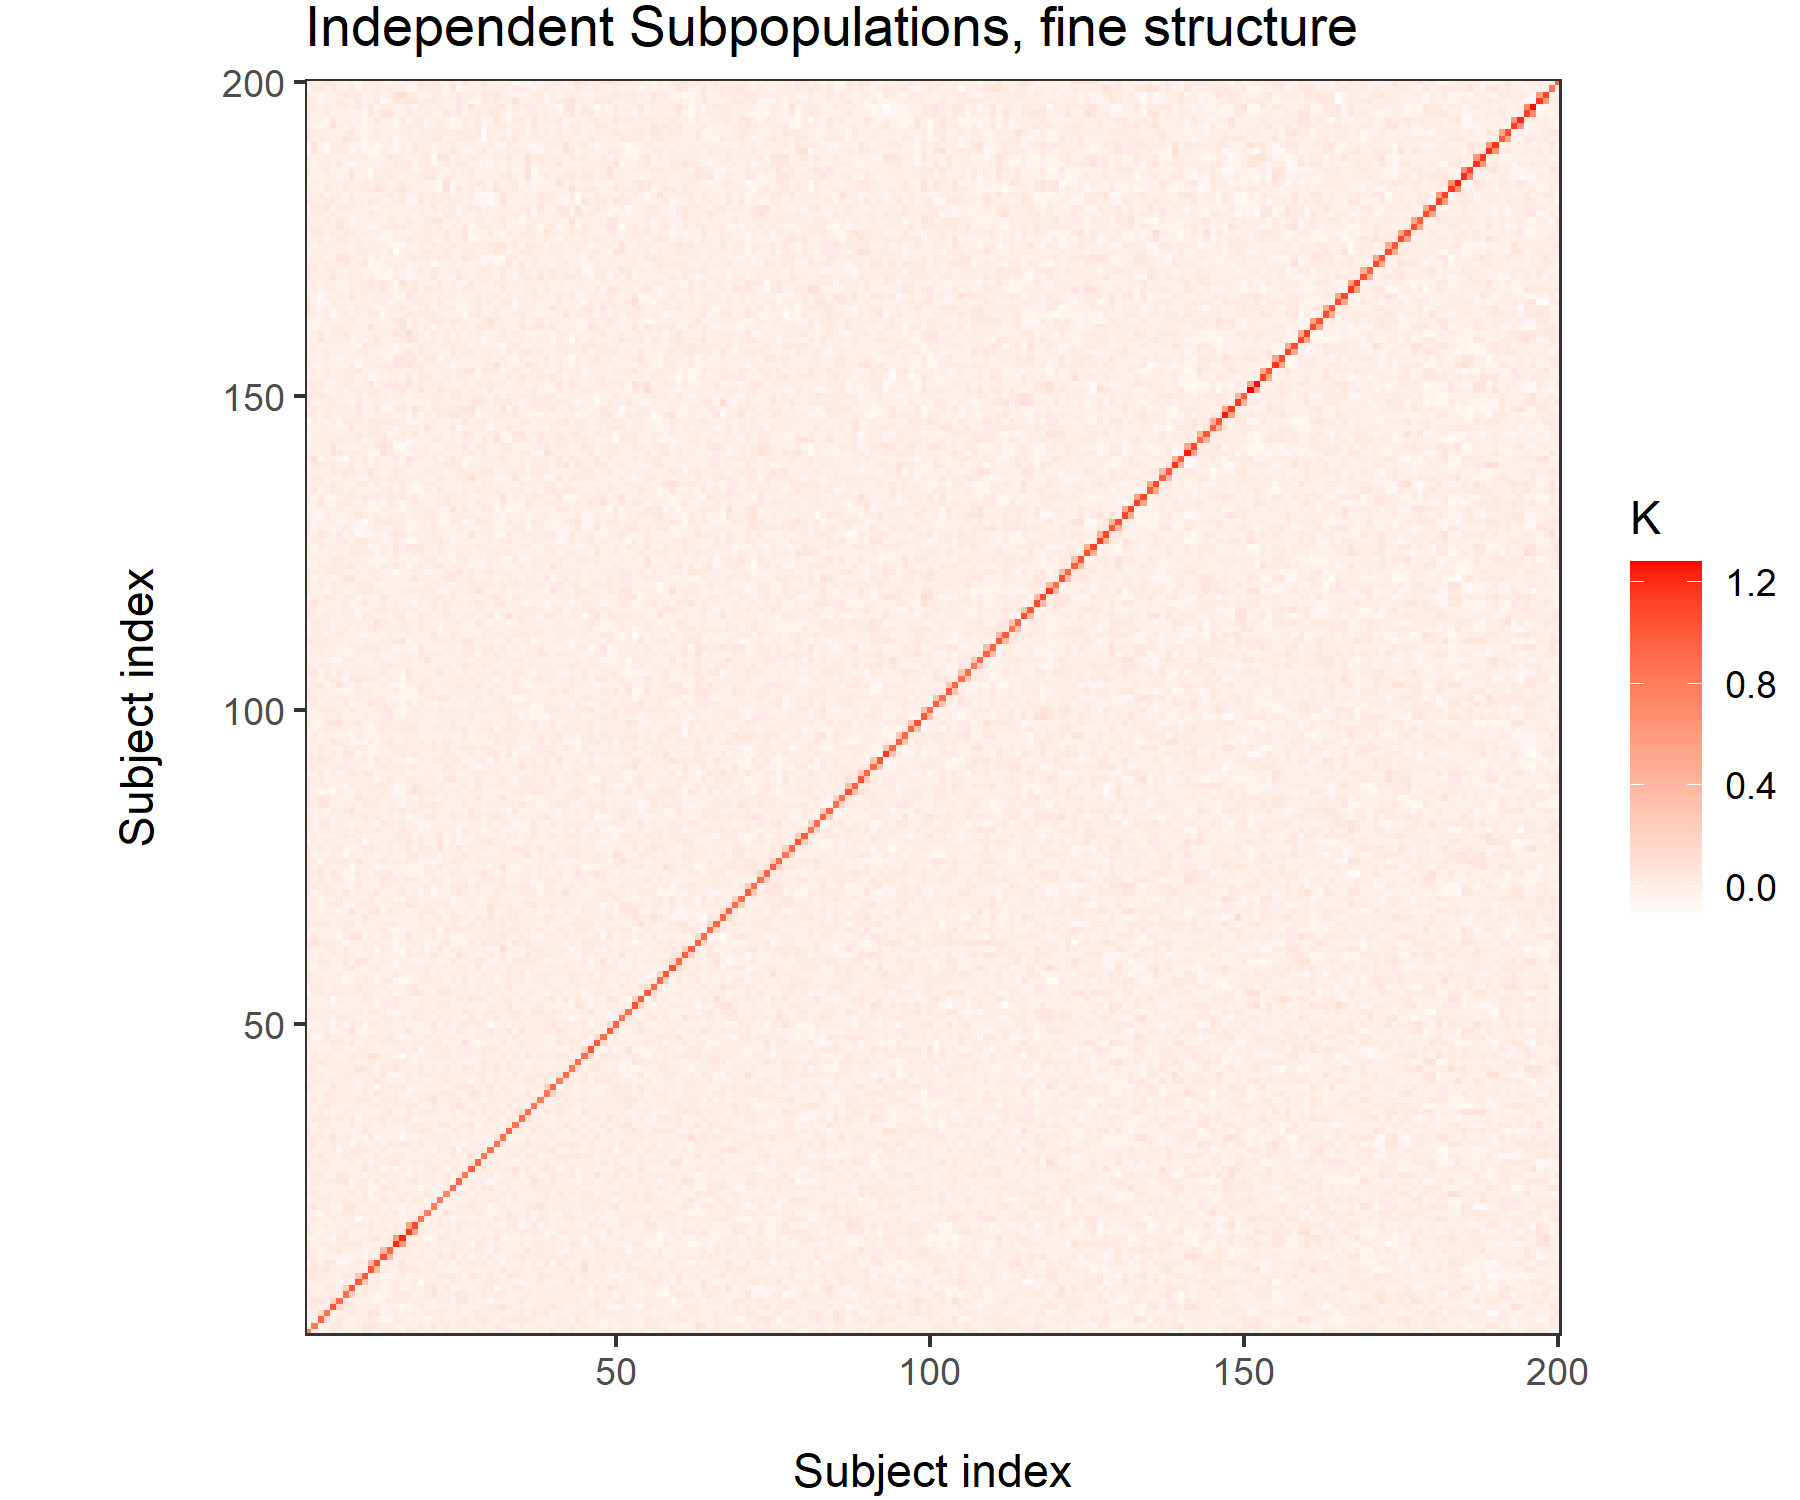
\includegraphics[scale = 1]{figures/indep_fine_kinship.png}
    \caption{Independent Subpopulations with fine subpopulation structure (2 subjects per subpopulation), RRM.}
    \label{fig:indep_fine}
\end{figure}

% EMPIRICAL KINSHIP
\begin{figure}[H]
    \centering
    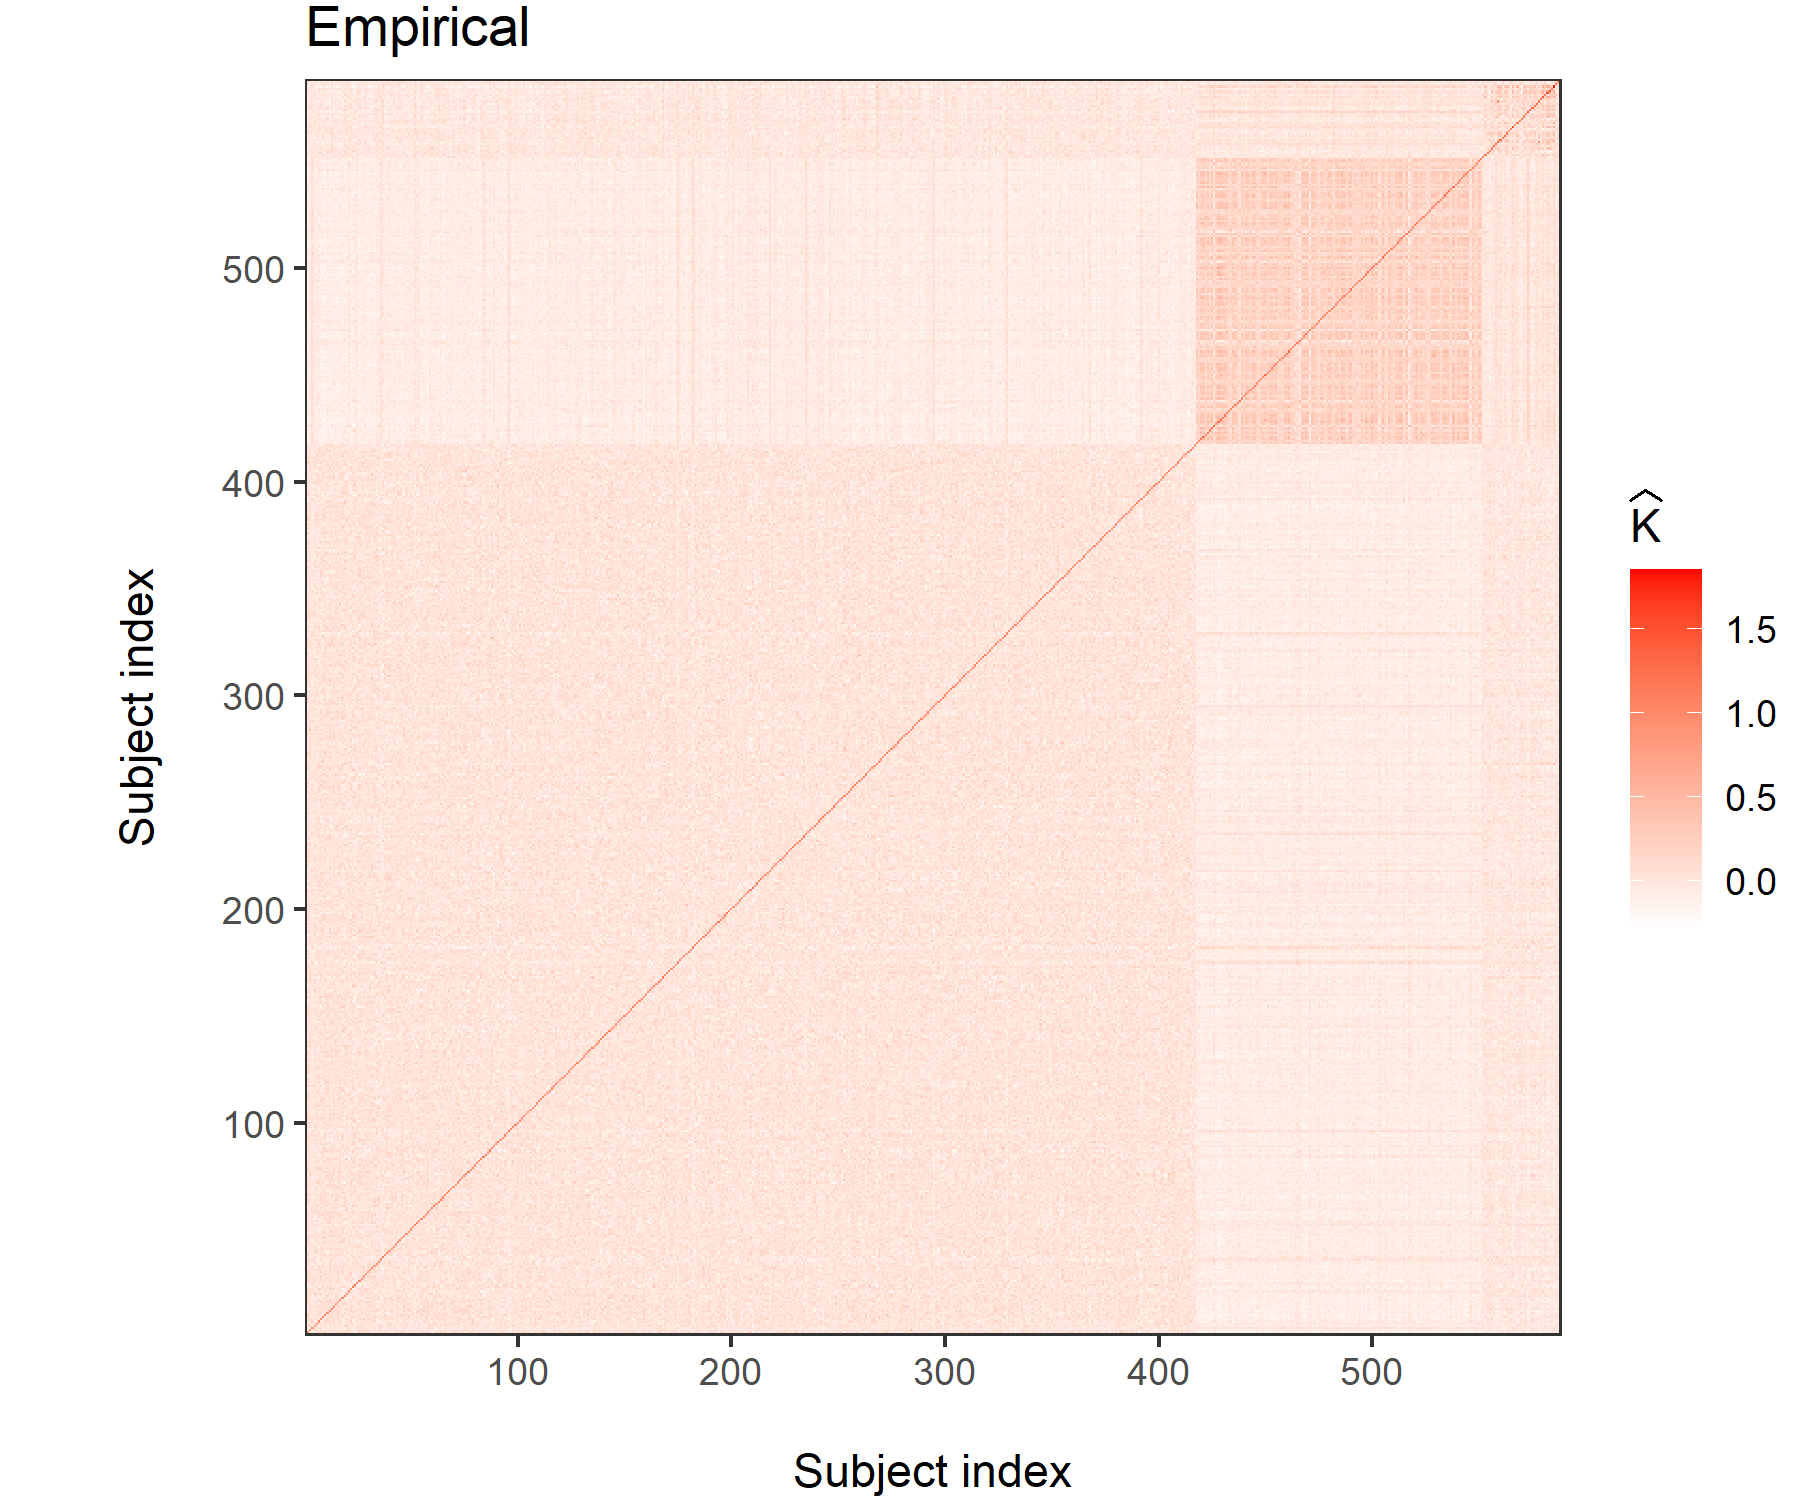
\includegraphics[scale = 1]{figures/empirical_kinship.png}
    \caption{Empirical RRM.}
    \label{fig:empirical}
\end{figure}

\begin{landscape}
\begin{figure}[H]
    \centering
    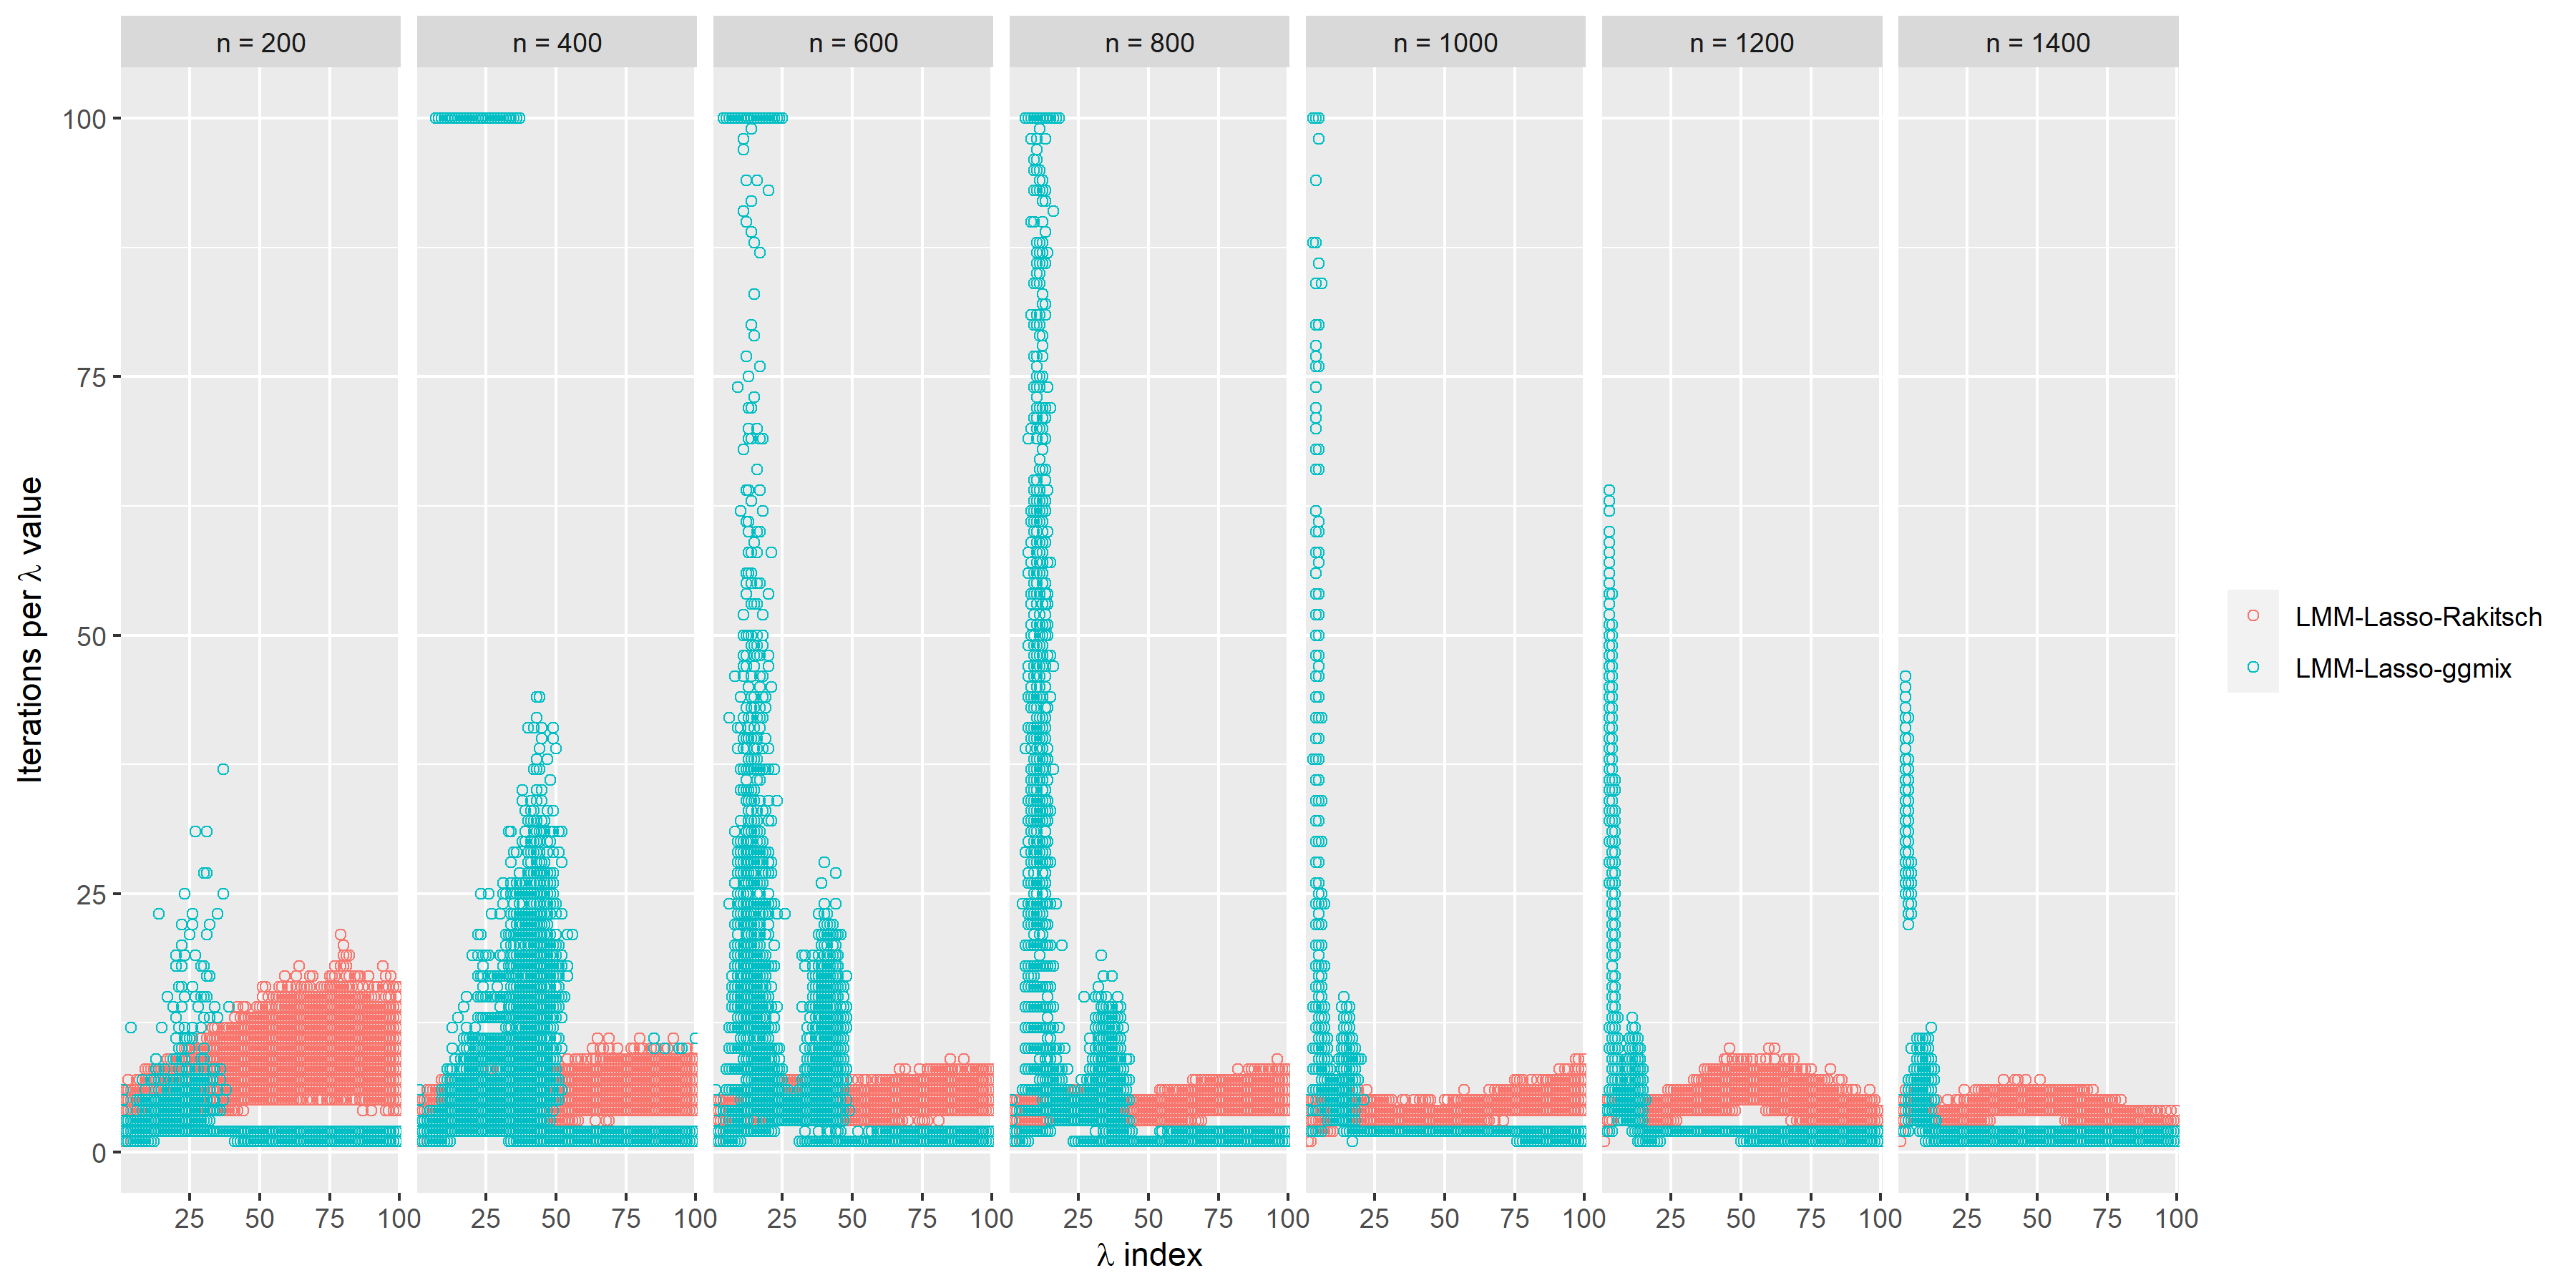
\includegraphics[scale = 0.8]{figures/niter_perLambda_point.png}
    \caption{The number of iterations per $\lambda$ value for LMM-Lasso-Rakitsch and LMM-Lasso-ggmix across varying sample sizes with Independent Subpopulations data, coarse subpopulation structure, $\eta = 0.8$, and $\xi = 0.8$, and dichotomous-discordant environmental effect structure. Note that 100 is the maximum number of iterations for both implementations of LMM-Lasso, so that numerous incidences of 100 iterations may indicate lack of model convergence.}
    \label{fig:niter}
\end{figure}
\end{landscape}